\documentclass[10pt,a4paper]{article}
\usepackage[utf8]{inputenc}
\usepackage{amsmath}
\usepackage{amsfonts}
\usepackage{amssymb}
\usepackage{graphicx}
\usepackage[swedish]{babel}
\usepackage[utf8]{inputenc}
\usepackage{amsmath}

\graphicspath{}

\author{
  \texttt{Sebastian Bångerius}
  \and
  \texttt{Andreas Nordberg}
  \and
  \texttt{Villiam Rydfalk}
  \and
  \texttt{Anton Silfver}
}

\begin{document}
\pagenumbering{gobble}

\title{Studsmatta}
\maketitle
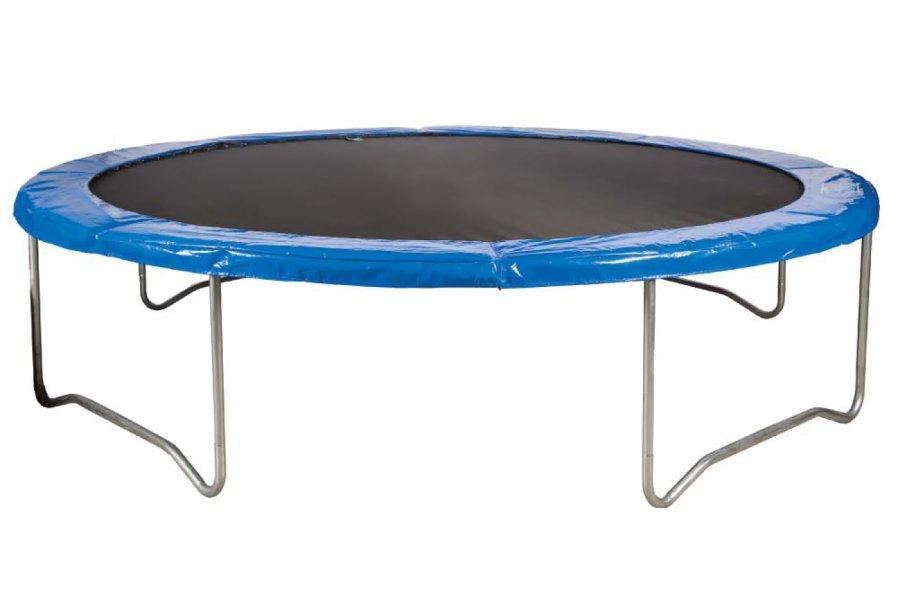
\includegraphics[scale=0.35]{Framsida}
\cleardoublepage

\tableofcontents

\clearpage

\section{Inledning}
\pagenumbering{arabic}
\setcounter{page}{3}

I den här rapporten kommer vi beskriva när en person sätter en studsmatta i rörelse som ett linjärt svängningssystem av andra ordningen. Inom det här systemet är insignalen kraften som personen trycker ifrån med när den sträcker ut eller böjer på benen, vilket resulterar i utsignalen som är studsmattans lägesändring ifrån sitt jämviktsläge, med positiv rikning mot marken. Genom att beskriva systemet med en differentialekvation av andra orningen kan vi få information om systemets egenskaper och dess beteende för olika insignaler, med andra ord hur olika faktorer påverkar utsignalen\cite[s.~57]{sune2000}.

\subsection{Syfte}
Syftet med den här rapporten är att utöka vår förståelse för hur linjära system fungerar och att få en uppfattning om hur den teorin vi lärt oss kan tillämpas i praktiken. Det är vår förhoppning att vi kan uppnå denna förståelse genom att modellera och analysera en studsmatta som ett linjärt system.

\subsection{Mål}
Målet med vår rapport är att förstå hur ett linjärt system kan fungera och påverkas, alltså hur insignalen till systemet kan ändras för att få utsignalen att bete sig på ett visst sätt. Ett exempel är hur insignalen kan påverkas för att få största möjliga utsignal, med andra ord att kunna hoppa så högt som möjligt på en studsmatta.

\section{Bakgrund}

Vi har i denna rapport valt att modellera en person som hoppar på en studsmatta som ett LTI (linjärt tidsinvariant) system för att undersöka dess egenskaper. Vi valde studsmattan för att få en verklighetsanknuten modell som inte kräver så mycket idealisering för att kunna representeras som ett linjärt svängningssystem.
\newpage

\subsection{Linjärt system}

Om vi antar att vårt system har en insignal $x(t)$ och en utsignal $y(t)$ så är vanlig notation att beteckna systemet med $x(t) \rightarrow y(t)$ \cite[s.~43]{sune2000}. Detta system kan ha flera egenskaper, men en vanlig egenskap som kännetecknar vårt svängande system är linjäritet. För att ett system ska vara linjärt måste det uppfylla två krav. Systemet måste dels vara homogent, d.v.s. uppfylla ekvationen:
\begin{equation}
a \cdot x(t) \rightarrow a \cdot y(t) 
\end{equation}
Systemet måste också vara additivt, d.v.s. uppfylla ekvationen:
\begin{equation}
x(t) = x_1(t) + x_2(t) \rightarrow y(t) = y_1(t) + y_2(t)
\end{equation}
Om man slår ihop ekvation 1 och 2 så kan man förkorta kravet till en ekvation:
\begin{equation}
x(t) = a \cdot x_1(t) + b \cdot x_2(t)\rightarrow y(t) = a \cdot y_1(t) + b \cdot y_2(t)
\end{equation}
\linebreak
Således måste alla linjära system uppfylla ekvation 3 \cite[s.~42]{sune2000}.
I vårt system betyder detta t.ex. att en speciellt stark kraft inte kommer förstöra fjädrarna.

%[Varför är vårt system linjärt? varför är det relevant och vilka konkreta egenskaper hos linjära system använder vi oss av]

\subsection{Tidsinvarians}

Ett system med insignal $x(t)$ och utsignal $y(t)$ sägs vara tidsinvariant om insignalen $x(t - \tau)$ ger upphov till utsignalen $y(t - \tau)$ \cite[s.~41]{sune2000}. Detta betyder alltså att de fysikaliska komponenterna i systemet inte varierar över tid. I vårt fall betyder det t.ex. att våra fjädrar inte slits ut och att personen som gungar inte byter plats på mattan. 

\newpage
\section{Vårt LTI system}
%ändra elsastisk till elastisk
\begin{figure}[ht]
\begin{center}
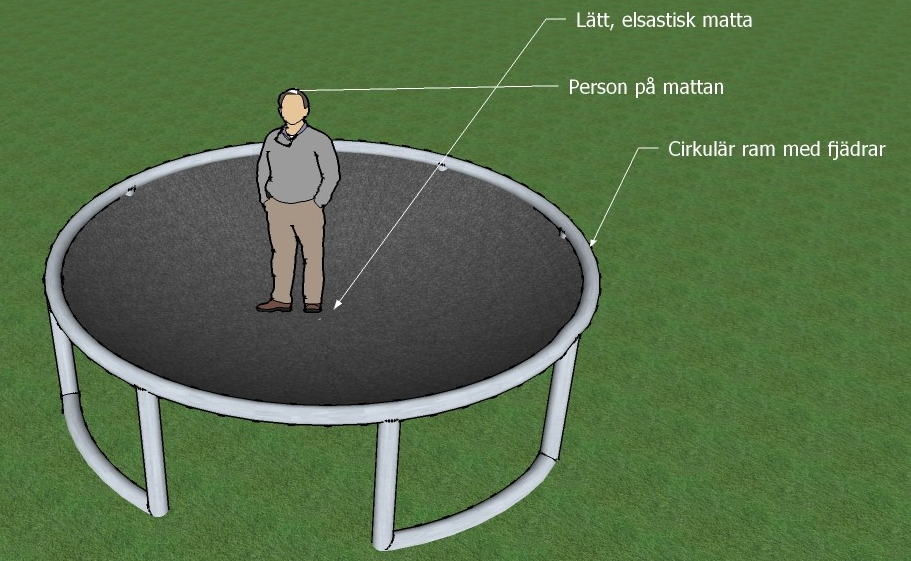
\includegraphics[scale=0.62]{Bild2}
\caption{En enkel bild av vårt system}
\end{center}
\end{figure}

Figur 1 ger en mycket enkel överblick av vårt system. Studsmattan är helt cirkulär och har fjädrar som sitter radiellt från kanten riktade in mot mitten, symmetriskt runt om hela cirkeln. Vi gör antagandet att personen som hoppar står precis i mattans mitt med fötterna tätt ihop (se figur 2). Mattan antas även vara fäst vid personens fötter, så att personen i själva verket inte hoppar utan bara gungar upp och ned genom att böja på benen. Med det menar vi att fötterna inte lämnar mattan

\subsection{Idealisering}
För att inte behöva räkna på varje individuell fjäder har vi valt att modellera systemet som \textit{en} enkel fjäder riktad vinkelrät mot markytan. Varför detta kan göras redovisas nedan:

\begin{figure}[ht]
\begin{center}
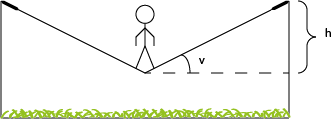
\includegraphics[scale=0.8]{fransidan}
\caption{En genomskärning från sidan}
\end{center}
\end{figure}
I figur 3 ses höjden $h$ samt vinkeln $v$. $h$ representerar höjdskilnaden från jämviktsläget då mattan är helt platt. $v$ är vinkeln på fjädern med avseende på nyss nämnda läge.
I och med att det för varje fjäder sitter en annan fjäder på motsatt sida studsmattan (enligt figur 3) kan vi modellera fjäderkrafterna som i figur 4.
\begin{figure}[ht]
\begin{center}
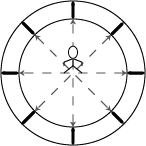
\includegraphics[scale=1]{ovanifran}
\caption{Vi ser hur det för varje fjäder finns ytterligare en, på motsatt sida}
\end{center}
\end{figure}

Vi tar nu en titt på de krafter som orsakas av ett fjäderpar ($F_1,F_2$). Dessa fjäderkrafter kan delas upp i komposanter:
\begin{figure}[ht]
\begin{center}
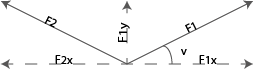
\includegraphics[scale=1]{krafter}
\caption{redovisning av krafter}
\end{center}
\end{figure}

Förutsatt att dessa fjädrar har samma fjäderkonstant och i sitt grundutförande är lika långa får vi sambanden:
$$F_1=k\Delta l_1\hat{f_1}, F_2=k\Delta l_2\hat{f_2}$$
Om nu $|\Delta l_1|=|\Delta l_2|$ kan vi konstatera att
$$F_{1x}=-F_{2x}, F_{1y}=F_{2y}$$
$$F_{tot}=F_1+F_2=(F_{1y}+F_{2y})\hat{y}=2k\Delta l\sin(v)\hat{y}$$

\pagebreak
Vi tar nu en titt på figur 5 som beskriver fjäderns utsträckning. Detta för att kunna uttrycka kraften som en funktion av $h$ och $k$ istället för $l$ och $k$.

\begin{figure}[ht]
\begin{center}
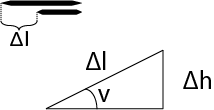
\includegraphics[scale=0.5]{utstrackning}
\caption{Utsträckning för en fjäder}
\end{center}
\end{figure}

$$\Delta h = \Delta l \sin(v) \rightarrow F_{tot}=2k\Delta l \sin(v)=2k\Delta h\propto k\Delta h $$

\begin{figure}[!h]
\begin{center}
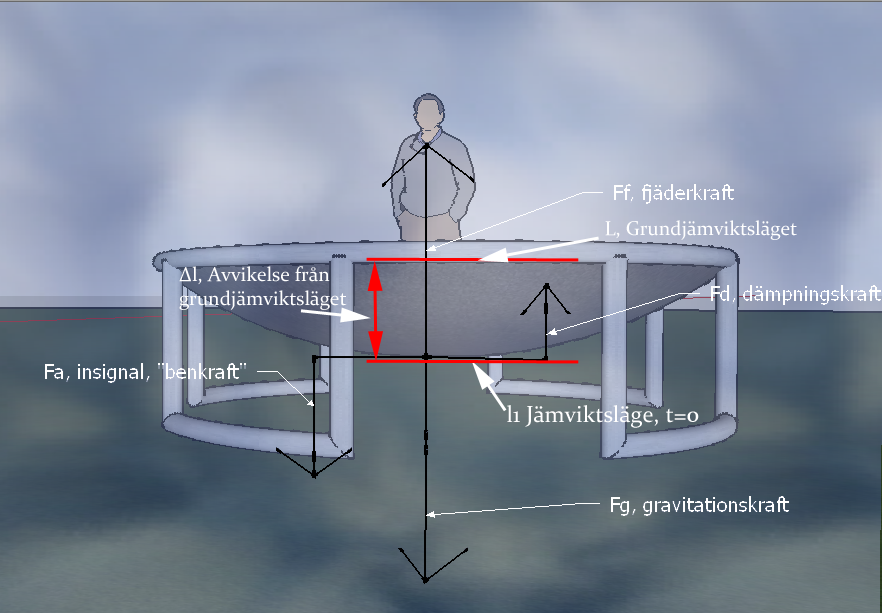
\includegraphics[scale=0.7]{KrafterIllustrationFinal}
\caption{Utsträckning för en fjäder}
\end{center}
\end{figure}

Vi kan alltså modellera vår studsmatta som en enkel fjäder som står på marken under den gungande personens fötter.
Insignalen i vårt system blir alltså kraften som den gungande personen utför på systemet då denne böjer eller sträcker på benen. Utsignalen i systemet definieras som mattans ändring i höjdled med referenspunkt i jämviktsläget på studsmattan, med positiv riktning mot marken. I bild X illustreras jämviktslägets ändring av massan.
%Jämviktsläget varierar i höjd beroende på massan som står på mattan.
%Uppdatera till att matcha den slutliga referensbilden
Krafterna uttryckta med pilar i figur 6 är gravitationskraften från massan $F_g$, fjäderns motkraft på massan $F_f$, fjäderns dämpningskraft $F_d$ och kraften från personen som trycker emot $F_a$.
Då fjädrarna i vår studsmatta är placerade symmetriskt och personen står placerad i mitten av mattan kan vi idealisera systemet som en enda fjäder verkande i y-led, eftersom de radiella krafterna tar ut varandra i symmetrin.


\subsection{Gravitationskraften $F_g$}

Gravitationskraften $F_g$ är den kraften som påverkar en massa $m$ med en konstant gravitationsacceleration $g$.

\begin{equation}
F_g = m  g
\end{equation}

\subsection{Fjäderkraften $F_f$}

Fjäderkraften $F_f$ är den kraft som motverkar en fjäders avskiljning ifrån sitt jämviktsläge. Sambandet har namnet Hookes lag 
\cite[s.~278]{randall2008}. Om fjäderns grund-\newline jämviktsläge är $L$ och dess jämviktsläge efter att massan läggs på är $l_1$ så kan vi uttrycka avvikelsen från grundjämviktsläget vid $t=0$ som $\Delta l = L - l_1$. Eftersom vi har avvikelsen från grundjämviktsläget $\Delta l$ så lägger vi på $y(t)$. Fjäderkonstanten sätts till $k$. Denna kraft är motriktad den av gravitationen och uttrycks på följande vis:

\begin{equation}
F_f = -k (\Delta l + y(t))
\end{equation}

\subsection{Dämpningskraften $F_d$}

Dämpningskraften $F_d$ är den kraft som motverkar rörelsen i ett svängningssystem där $v$ är objektet i rörelses momentana hastighet och $c$ är dämpningskoefficienten för svängningsrörelsen. Dämpningskraften är motriktad rörelsen.

\begin{equation}
F_d = -c  v
\end{equation}

\subsection{Slutgiltig differentialekvation}

Systemet består av de åvanstående tre krafterna samt insignalen som alla är krafter i y-led. Summan av dessa krafter skapar den totala kraften $F_{tot}$. Vi kan då beskriva vårt system med följande ekvation:

\begin{equation}
F_{tot} = F_a + F_g + F_f + F_d
\end{equation}

Vi sätter $F_a$ som insignalen $x(t)$ vilket tillsammans med våra tidigare definitioner och Newtons andra lag \cite[s.~138]{randall2008} ger:

\begin{equation}
F_{tot} = x(t) + mg - k(\Delta l+y(t)) - cv = ma
\end{equation}

Vi uttrycker hastighet och acceleration som funktioner av $t$:
\begin{equation}
a = \frac{d^2y(t)}{dt^2} , v = \frac{y(t)}{dt}
\end{equation}

Vilket ger:

\begin{equation}
 m\frac{d^2y(t)}{dt^2} =  -k(\Delta l + y(t)) -c\frac{dy(t)}{dt} + mg +  x(t)
\end{equation}

Gravitationen $mg$ är alltid i positiv riktning (mot marken) och fjäderkraften $F_f$ kommer vara i antingen positiv eller negativ riktning beroende på insignalen. Vid $t = 0$ så står systemet still i jämviktsläget. Personen gungar inte. Det vill säga ingen insignal och ingen utsignal. Detta kan bara ske om gravitationskraften och kraften från fjäderns utsträckning tar ut varandra. Alltså:
\begin{equation}
k \Delta l = mg
\end{equation}

Vilket ger vår slutgiltiga differentialekvation:
\begin{equation}
 m\frac{d^2y(t)}{dt^2} + k  y(t) + c\frac{dy(t)}{dt} = x(t)
\end{equation}
\newpage

\section{Systemegenskaper}

Vårt system kommer ha en lång rad egenskaper som definerar systemet. I följande kapitel så kommer vi analysera några egenskaper som vi anser vara relevanta att studera och för att förstå hur vårt system beter sig. Egenskaperna kommer att bevisas och motiveras.

\subsection{Linjäritetsbevis}

För att visa att vårt system är linjärt måste vi visa att det är både homogent och additivt \cite[s.~42]{sune2000}, som nämnt tidigare. Om vi antar att insignalen $x_1(t) \rightarrow y_1(t)$ och $x_2(t) \rightarrow y_2(t)$ så gäller att:

\begin{equation}
m\frac{d^2y_1(t)}{dt^2} + c\frac{dy_1(t)}{dt} + ky_1(t) = x_1(t)
\end{equation}

\begin{equation}
m\frac{d^2y_2(t)}{dt^2} + c\frac{dy_2(t)}{dt} + ky_2(t) = x_2(t)
\end{equation}


Om vi då låter insignalen vara $a_1 x_1(t) + a_2 x_2(t)$ där $a_1$ och $a_2$ är reella konstanter så ger det:
\begin{equation}
m\frac{d^2y(t)}{dt^2} + c\frac{dy(t)}{dt} + ky(t) = a_1 x_1(t) + a_2 x_2(t)
\end{equation}

Ekvation 13, 14 och 15 ger:

\begin{equation}
\begin{split}
m\frac{d^2y(t)}{dt^2} + & c\frac{dy(t)}{dt} + ky(t) = \\ = a_1(m\frac{d^2y_1(t)}{dt^2} + c\frac{dy_1(t)}{dt} +  ky_1(t)) & + a_2(m\frac{d^2y_2(t)}{dt^2} + c\frac{dy_2(t)}{dt} + ky_2(t))
\end{split}
\end{equation}

Högerledet i ekvation 12 kan skrivas:

\begin{equation}
m\frac{d^2\{a_1y_1(t) + a_2y_2(t)\}}{dt^2} + c\frac{d\{a_1y_1(t) + a_2y_2(t)\}}{dt} + k\{a_1y_1(t) + a_2y_2(t)\}
\end{equation}

Vilket ger:
\begin{equation}
\begin{split}
m\frac{d^2y(t)}{dt^2} +  cm\frac{dy(t)}{dt} + ky(t) = & \\ = m\frac{d^2\{a_1y_1(t) + a_2y_2(t)\}}{dt^2} + c\frac{d\{a_1y_1(t) + a_2y_2(t)\}}{dt} + & k\{a_1y_1(t) + a_2y_2(t)\}
\end{split}
\end{equation}

Alltså:

\begin{equation}
y(t) = a_1 y_1(t) + a_2 y_2(t)
\end{equation}

Systemet uppfyller således kravet för linjäritet.





\subsection{Systemfunktionen}

Systemfunktionen är mycket relevant hos ett system och ger information om en rad olika följdegenskaper som t.ex. stabilitet och kausalitet, om systemet filtrerar ut låga eller höga frekvenser och mycket annat \cite[s.~170]{sune2000}. Vi vill ta fram systemfunktionen för att andra ta fram egenskaperna hos vårt system.

Med differentialekvationen kan vi genom laplacetransformering ta fram systemfunktionen $H(s)$. Laplacetransform är en matematisk transform som tar en funktion av tiden till frekvensdomänen. %Här ska det vara mer om laplacetransform!!!

\begin{equation}
\begin{split}
 m\frac{d^2y(t)}{dt^2} + k  y(t) + c\frac{dy(t)}{dt} & = x(t) \\ \leftrightarrow m  s^2  Y(s) + c  s  Y(s) + k  Y(s) & = X(s)
\end{split}
\end{equation}

Bryter vi ut $Y(s)$ i vänsterledet får vi:

\begin{equation}
Y(s)(m  s^2 + c  s + k) = X(s)
\end{equation}

Eftersom $H(s) = \frac{Y(s)}{X(s)}$ så flyttar vi om och får:

\begin{equation}
H(s) = \frac{Y(s)}{X(s)} = \frac{1}{m s^2 + c  s + k}
\end{equation}

Om vi tar fram rötterna till nämnaren får vi:

\begin{equation}
H(s)= \frac{1}{(s + \frac{c}{2 m} + \sqrt{ (\frac{c}{2  m})^2 - \frac{k}{m}}) (s + \frac{c}{2  m} - \sqrt{ (\frac{c}{2  m})^2 - \frac{k}{m}})}
\end{equation}

Poler produceras där nämnarpolynomet har sina rötter:

\begin{equation}
S_{rot}=-\frac{c}{2m} \pm \sqrt{(\frac{c}{2m})^2-\frac{k}{m}}
\end{equation}

Vi ser att vi antingen kan få två komplexa rötter, en reell dubbelrot, eller två reella rötter. Vi har alltså tre distinkt olika sätt som våra poler kan placera sig på enligt följande:
\begin{itemize}

\item $H(s)$ har en dubbelrot om $\sqrt{(\frac{c}{2m})^2-\frac{k}{m}}=0$ (Då är $S_{rot}=-\frac{c}{2m}$)


\item $H(s)$ har två rella rötter om $0\neq\sqrt{(\frac{c}{2m})^2-\frac{k}{m}}\in \mathbb{R}$ \newline d.v.s. om $(\frac{c}{2m})^2-\frac{k}{m}>0$


\item $H(s)$ har två komplexa rötter om $\sqrt{(\frac{c}{2m})^2-\frac{k}{m}}\notin \mathbb{R}$ \newline d.v.s. om $(\frac{c}{2m})^2-\frac{k}{m}<0$

\end{itemize}

Detta kan illustreras och förenklas till (figur 7-9):

\begin{figure}
\begin{center}
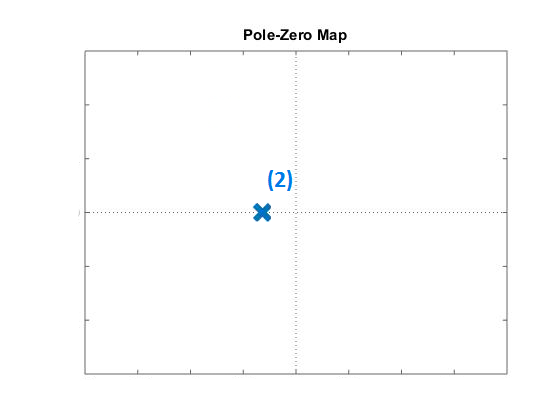
\includegraphics[scale=0.6]{1reell}
\caption{Dubbelpol $s_{rot}=-\frac{c}{2m}$ om $k=\frac{c^2}{4m}$}
\end{center}
\end{figure}

\begin{figure}
\begin{center}
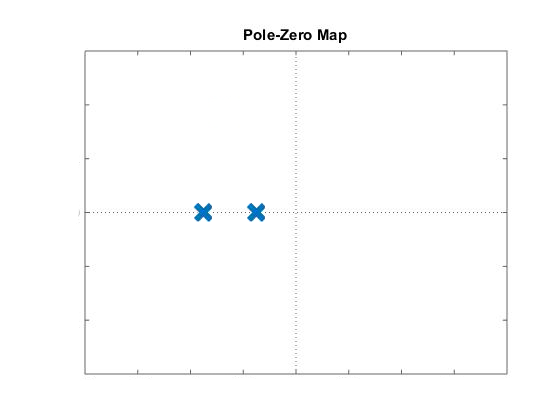
\includegraphics[scale=0.3]{2reella}
\caption{Två reella poler om $k<\frac{c^2}{4m}$}
\end{center}
\end{figure}

\begin{figure}
\begin{center}
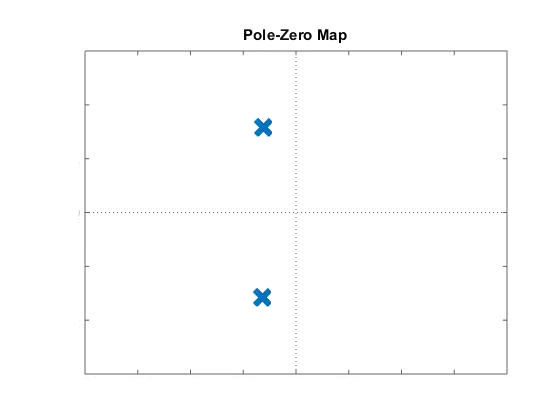
\includegraphics[scale=0.3]{2komplexa}
\caption{Två komplexa poler om $k>\frac{c^2}{4m}$}
\end{center}
\end{figure}
\newpage


I vårt fall med studsmattan vill vi gärna skapa så hög amplitud ut som möjligt, med mycket svängning och lite dämpning. Detta återfinns i det tredje fallet med två komplexa rötter och brukar kallas för ett underdämpat system \cite{polesAndZeros}. Det kan visualiseras grafiskt i form av amplitudkaraktäristik, som visas i figur 14 senare i rapporten. Nedan i figur 10 visas ett pol/nollställe-diagram över vårt system med följande konstanter insatta $k=2000\frac{N}{m}$ , $m=70kg$ , $c=100\frac{kg}{s}$. Dessa konstanter valdes inte helt slumpmässigt. Vi valde $k = 2000$ för att då krävs det en kraft av 1000 N för att dra ned fjädern en halvmeter, det vill säga en person som väger 100 kg skulle sjunka ned ungefär en halvmeter om denne stod på studsmattan. Detta anser vi relativt rimligt. Personen som hoppar väger 70 kg vilket är en ganska vanlig vikt hos en normalstor person. Dämpningskonstanten är den som var svårast att välja, och beroende på dess värde får systemet väldigt olika egenskaper. Konstanten c är mer eller mindre omöjlig för oss att resonera oss fram till en vettig siffra, så vi valde 100 för att det gav oss värden som ser helt okej ut för en studsmatta. Figur 11 visar en 3D-plot utav vår systemfunktionen.


\begin{figure}[h]
\begin{center}
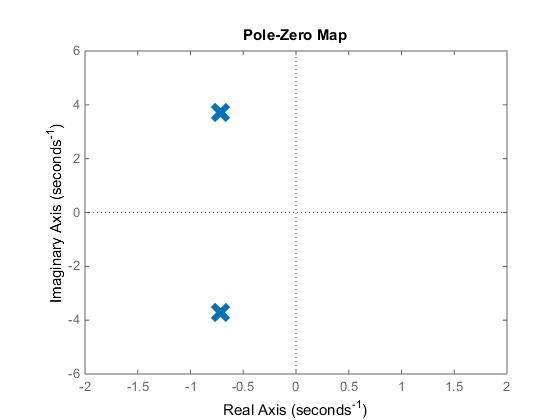
\includegraphics[scale=0.4]{nolpol-diagram}
\caption{$s = -0,714 \pm 3,712j$}
\end{center}
\end{figure}
\begin{figure}[h]
\begin{center}
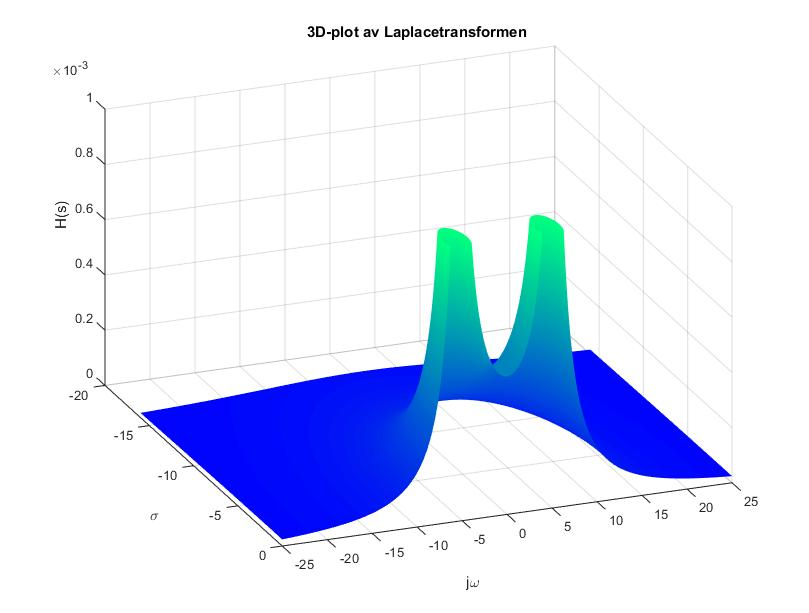
\includegraphics[scale=0.25]{3Dpoler5}
\caption{3D-representation av laplacetransformen för vårt system}
\end{center}
\end{figure}

\newpage


\subsection{Impulssvar}

Genom att kvadratkomplettera $H(s)$ får vi:

\begin{equation}
H(s) = \frac{1}{m} \cdot \frac{1}{(s+(\frac{c}{2  m}))^2-(\frac{c}{2  m})^2+\frac{k}{m}} 
\end{equation}

Om vi sätter $\alpha = \frac{c}{2m}$ och $\omega_0^2 = {-\frac{c + 4 k  m^2}{4  m^2}}$ och förlänger med $\frac{\omega_0}{\omega_0}$ får vi:

\begin{equation}
H(s) = \frac{1}{\omega_0  m} \cdot \frac{\omega_0}{(s + \alpha)^2 +\omega_0^2}
\end{equation}

Genom att inverslaplacetransformera $H(s)$ får vi impulssvaret $h(t)$ \cite[s.~207]{sune2000}. Vi använder tabell 19.23 i Sune Söderkvist formelsamling:

\begin{equation}
\begin{split}
h(t) = \frac{1}{\omega_0  m} \cdot  e^{-\alpha  t} & \cdot  sin(\omega_0  t) \cdot u(t) = \\ = \frac{1}{\sqrt{\frac{4  m  k - c^2}{4}} } \cdot  e^{-\frac{c}{2m} t} \cdot & sin(\sqrt{\frac{4  m  k - c^2}{4  m^2}} \cdot t) \cdot u(t)
\end{split}
\end{equation}



\begin{figure}[h]
\begin{center}

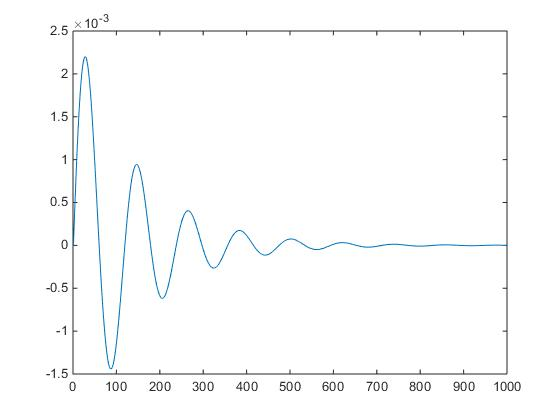
\includegraphics[scale=0.5]{Impulssvar}
\caption{Vårt systems impulssvar}
\end{center}
\end{figure}



\newpage
\subsection{Stabilitetsbevis}
För att vår idealisering skall vara representativ för vår studsmatta måste systemet vara stabilt. Vi får stabilitet om $\int_{-\infty}^{\infty}|h(t)|\ dt\in \mathbb{R}$ \cite[s.~48]{sune2000}. I grund och botten betyder detta att vårt system ej får tillföra mer energi än vad som läcker ut. Nedan följer en förenkling av integralen:
\begin{equation}
\begin{split}
I_{impuls}=\int_{-\infty}^{\infty}| \frac{1}{\sqrt{\frac{4  m  k - c^2}{4}} }  \cdot e^{-\frac{c}{2m}  t} \cdot & sin(\sqrt{\frac{4  m  k - c^2}{4  m^2}} \cdot t) \cdot u(t)| \ dt=\\ \frac{1}{\sqrt{\frac{4  m  k - c^2}{4}} }  \cdot \int_{0}^{\infty}|e^{-\frac{c}{2m}  t}| \cdot & |sin(\sqrt{\frac{4  m  k - c^2}{4  m^2}} \cdot t)| \ dt
\end{split}
\end{equation}
Förenklingar för att göra beviset mer lättläsligt:
\begin{itemize}
\item $\omega_0=\sqrt{\frac{4  m  k - c^2}{4  m^2}}$
\item $\alpha=\frac{c}{2\cdot m}$
\item $\omega_1=\sqrt{\frac{c^2-4  m  k}{4  m^2}}$
\newline
\newline 
Notera att: $\left( \omega_0=\sqrt{\frac{4  m  k-c^2}{4  m^2}}=\sqrt{(-1)\cdot\frac{c^2-4  m  k}{4  m^2}}=i\cdot\sqrt{\frac{c^2-4  m  k}{4  m^2}}=i \omega_1\right)$
\end{itemize}

Vi konstaterar att delfunktionerna är positiva för alla positiva $t$. Således är även integralen av produkten det:
$$I_{impuls}=\frac{1}{\omega_0  m} \cdot \int_{0}^{\infty}e^{-\alpha t}\cdot | sin(\omega_0 t)| \ dt>0$$

Vi bevisar att integralen är begränsad för tre olika fall: då $0\neq\omega_0 \in \mathbb{R}$, $\omega_0=0$ respektive då $\omega_0 \notin \mathbb{R}$

\begin{itemize}
\item fallet $k>\frac{c^2}{4m}$ ($0\neq\omega_0 \in \mathbb{R}$, underdämpat system)
\begin{equation}
\begin{split}
I_{impuls}=\frac{1}{\omega_0  m} \cdot \int_{0}^{\infty}e^{-\alpha t}\cdot & | sin(\omega_0 t| \ dt <\frac{1}{\omega_0  m}\int_{0}^{\infty}e^{-\alpha t} \  dt =\\\frac{1}{\omega_0  m} \cdot \left[\frac{-e^{-\alpha t}}{\alpha}\right]_0^\infty= \frac{1}{\omega_0  m} & \cdot \frac{1}{\alpha}=\frac{1}{\sqrt{\frac{4 m k- c^2}{4}}\cdot\frac{c}{2m}}\in \mathbb{R}^+
\end{split}
\end{equation}
\item fallet $k=\frac{c^2}{4m}$ ($\omega_0=0$, kritiskt dämpat system)
\newline 
Här får vi problem med att faktorn framför integralen blir odefinierad samtidigt som sinusen blir 0. Vi använder oss av gränsvärdesanalys för att lösa det problemet.
\begin{equation}
\begin{split}
I_{impuls}= & \lim_{\omega_0\to0}\left(\frac{1}{m} \cdot \int_{0}^{\infty}e^{-\alpha t}\cdot |\frac{sin(\omega_0 t)}{\omega_0}| \ dt\right) = \\ \frac{1}{m} &\cdot\int_{0}^{\infty}e^{-\alpha t} \cdot t  \  dt=...=\frac{4m}{c^2}\in \mathbb{R}^+
\end{split}
\end{equation}
Vi ser att vi intressant nog inte bara kan stänga in denna integral, utan faktiskt räkna ut ett värde för den.
\item fallet $k<\frac{c^2}{4m}$ ($\omega_0 \notin \mathbb{R}$, överdämpat system)
\newline Här råkar vi på ett annat problem: $\omega_0$ blir komplex. Således blir det svårt att integrera uttrycket. Vi tar nu hjälp av $\omega_1$.

\begin{equation}
\begin{split}
I_{impuls}= & \int_{0}^{\infty}\left|\frac{e^{-\alpha t}}{\omega_0  m}\cdot sin(\omega_0 t)\right| \ dt=\\ & \int_{0}^{\infty}\left|\frac{e^{-\alpha t}}{i\omega_1 m}\cdot i sinh(\omega_1 t)\right| \ dt=\\ & \frac{1}{\omega_1  m} \cdot \int_{0}^{\infty}\left|e^{-\alpha t}\cdot sinh(\omega_1 t)\right| \ dt=\\ & \frac{1}{2 \omega_1  m} \cdot \int_{0}^{\infty}e^{-\alpha t} \left( e^{\omega_1 t}-e^{-\omega_1 t} \right) \ dt< \\ & \frac{1}{2\omega_1  m} \cdot \int_{0}^{\infty}e^{(\omega_1-\alpha) t} \  dt=\frac{1}{2\omega_1  m}\left[\frac{e^{(\omega_1-\alpha) t}}{\omega_1-\alpha} \right]_{0}^{\infty}=\\ & \frac{1}{2\omega_1  m}\cdot\left(\frac{-1}{\omega_1-\alpha} \right)=\frac{1}{2\omega_1  m} \cdot \left(\frac{1}{\alpha-\omega_1} \right)=\\ & \frac{1}{2 \sqrt{\left(\frac{c}{2 m}\right)^2-\frac{k}{m}}   \cdot m} \cdot \left(\frac{1}{\sqrt{\left(\frac{c}{2 m}\right)^2}-\sqrt{\left(\frac{c}{2 m}\right)^2-\frac{k}{m}}} \right)\in \mathbb{R}^+
\end{split}
\end{equation}
\end{itemize}

\newpage

\subsection{Stegsvar}
Ett stegsvar är en omedelbar upptrappning av insignalen till ett konstant värde. Detta kan approximativt motsvaras att personen som står på mattan får en omedelbar ökning av massan. T.ex. om personen fångar ett tungt objekt.

Vi vill ta fram stegsvaret $g(t)$ för vårt system. Vi gör detta genom att integrera vårt impulssvar upp till tiden $\tau$ $\int_{-\infty}^\tau h(t)$, vi börjar med att bryta ut våra konstanter utanför integralen. Vi räknar sedan ut integralen och till sist stoppar vi in konstanterna igen.

\begin{equation}
\int_{-\infty}^\tau \frac{1} {\omega_0 m} \cdot e^{-\alpha  t} \cdot sin(\omega_0  t) \cdot u(t) \  dt = \frac{1}{\omega_0  m} \cdot \int_{-\infty}^\tau sin(\omega_0 t)\cdot e^{-\alpha  t} \cdot u(t) \  dt
\end{equation}
Vi delar upp integralen i två integraler. Den ena för negativa $t$ den andra för positiva $t$ det ger:
$$ \int_{-\infty}^\tau sin(\omega_0  t)\cdot e^{-\alpha t} \cdot u(t)  \ dt
= \int_{-\infty}^0 sin(\omega_0  t)\cdot e^{-\alpha  t} \cdot u(t) \  dt + \int_0^\tau sin(\omega_0  t)\cdot e^{-\alpha  t} \cdot u(t) \  dt $$
Eftersom $u(t)$ är 0 för negativa $t$ och 1 för positiva $t$ vilket ger:
\begin{equation}
\int_{-\infty}^\tau sin(\omega_0  t)\cdot e^{-\alpha  t} \cdot u(t) \  dt
= \int_0^\tau sin(\omega_0  t)\cdot e^{-\alpha t} \  dt
\end{equation}
Vi låter integralen heta $I$ och räknar ut den:

\begin{equation}
\begin{split} 
I & = \int_0^\tau sin(\omega_0 t)\cdot e^{-\alpha t} \  dt  \\
& = [-\frac{1}{\omega_0} \cdot cos(\omega_0 t) \cdot e^{-\alpha t}]_0^\tau - \int_0^\tau \frac{\alpha}{\omega_0} \cdot cos(\omega_0 t) \cdot e^{-\alpha t}  \ dt \\
& = [-\frac{1}{\omega_0} \cdot cos(\omega_0 t) \cdot e^{-\alpha t}]_0^\tau - \\
& \frac{\alpha}{\omega_0} \cdot ([\frac{1}{\omega_0} \cdot sin(\omega_0 t) \cdot e^{-\alpha t}]_0^\tau - \int_0^\tau -\frac{\alpha}{\omega_0} \cdot sin(\omega_0  t)\cdot e^{-\alpha t}  \ dt \\
\leftrightarrow
I & = [-\frac{1}{\omega_0} \cdot cos(\omega_0 t) \cdot e^{-\alpha t}]_0^\tau - \frac{\alpha}{\omega_0} \cdot ([\frac{1}{\omega_0} \cdot sin(\omega_0 t) \cdot e^{-\alpha t}]_0^\tau - (\frac{\alpha}{\omega_0})^2 I \\
\leftrightarrow I & = \frac{1-cos(\omega_o \tau) \cdot e^{\alpha \tau} - \frac{\alpha}{\omega_0^2} \cdot sin(\omega_o \tau) \cdot e^{\alpha \tau}}{\omega_0 + \frac{\alpha^2}{\omega_0}}
\end{split}
\end{equation}

Vi stoppar ni in de konstanter vi bröt ut ur integralen tidigare för att få stegsvaret det ger:

\begin{equation}
g(\tau)= \frac{1}{\omega_ m} \cdot I = \frac{1-cos(\omega_o \tau) \cdot e^{-\alpha  \tau} - \frac{\alpha}{\omega_0^2} \cdot sin(\omega_o \tau) \cdot e^{-\alpha \tau}}{m (\omega_0^2 + \alpha^2)}
\end{equation}
I figur 13 så plottar vi stegsvaret
\newpage



Om vi låter $\tau \to \infty$ ger det:

\begin{equation}
g(\tau) = \lim_{\tau \to \infty} \frac{1 - cos(\omega_0 \tau) \cdot e^{-\alpha \tau}
- \frac{\alpha}{\omega_0^2} \cdot sin(\omega_0  \tau) \cdot e^{-\alpha  \tau}}{m  (\omega_o^2 +\alpha^2)}, \tau \to \infty
\end{equation}

Vi kan se att $e^{-\alpha  \tau} \to 0$ för $\tau \to \infty$ vilket ger:

\begin{equation}
g(\tau) = \frac{1}{m  (\omega_o^2 +\alpha^2)} , \tau \to \infty
\end{equation}

\begin{figure}
\begin{center}
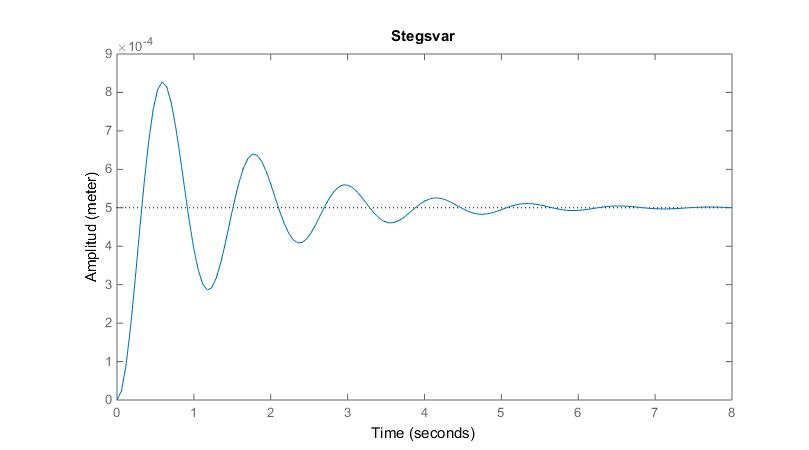
\includegraphics[scale=0.5]{Stegsvar}
\caption{Vårt systems stegsvar}
\end{center}
\end{figure}

\subsection{Frekvensfunktion}
Eftersom vårt system är stabilt kan vi enkelt översätta systemfunktionen till systemets frekvensfunktion \cite[s.~130]{sune2000}. Eftersom $s = \sigma + j\omega$ så kommer $\sigma = 0$ vid $j\omega$-axeln. Då följer att:

\begin{equation}
H(\omega) = H(s), \  s = j\omega
\end{equation}

Då följer det att vår frekvensfunktion är:

\begin{equation}
H(\omega) =  \frac{1}{m (j\omega)^2 + c  j\omega + k}
\end{equation}

\newpage
\subsection{Amplitud- och faskaraktäristik}

Amplitud och faskaraktäristik beskriver hur ett system påverkar en signals amplitud och fas beroende på frekvensen. Utsignalen har en amplitud som är insignalens amplitud multiplicerat med systemets amplitudkaraktäristik och utsignalens fasförskjutning bestäms utav systemets faskaraktäristik.

För att ta fram amplitudkaraktäristiken tar man absolutbeloppet av systemets frekvensfunktion, d.v.s. $|H(\omega)|$. Faskaraktäristiken får man genom att ta argumentet av frekvesnsfunktion, $arg(H(\omega))$\cite[s.~130]{sune2000}. 

\begin{equation}
|H(\omega)| = \frac{1}{|70 (j\omega)^2 + 100  j\omega + 2000|}
\end{equation}

MatLab har en inbyggd funktion för att rita amplitud- och fas-karaktäristik som kallas BodePlot. Ett Bodediagram är en graf för systemfunktioner där amplitud- och fas ritas som funktion av frekvens med logaritmisk skala.

Vår amplitud- och fas-karaktäristik med instoppade värden visas i bodediagrammet nedan:


\begin{figure}[h]
\begin{center}
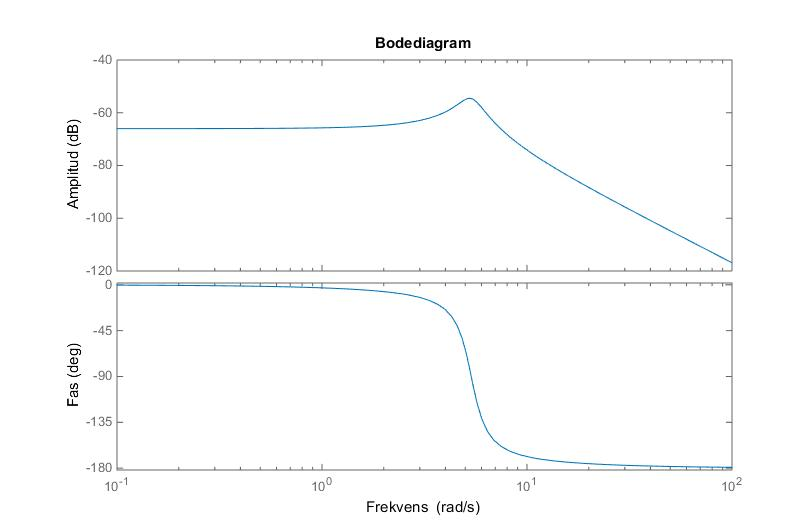
\includegraphics[scale=0.5]{BodePlot(FasAmpKar)}
\caption{$|H(\omega)| \ resp. \ arg(H(\omega)), k = 2000, c = 100 och m = 70$ }
\end{center}
\end{figure}

\newpage


\subsection{Resonansfrekvens}
I detta avsnitt diskuterar vi hur resonansfrekvensen beter sig i vårt system. Resonansfrekvensen är den frekvens på insignalen som leder till maximal amplitud på utsignalen\cite[s.~206]{sune2000}. I vårt fall med studsmattan är denna frekvens eftertraktad; den gör ju så att man gungar så högt som möjligt. Vi har framställt ett uttryck för resonansfrekvensen i vårt system genom att derivera amplitudkaratäristiken. Vi gör detta för att derivatan (lutningen) blir 0 då vi nått globalt maximum för amplitudkaraktäristiken.
\begin{equation}
\begin{split}
\omega=\omega_{res} \rightarrow \frac{d}{d\omega}\left|H(\omega)\right|=0\rightarrow \\ 
\frac{d}{d\omega}\left(\frac{1}{\left|-\omega^2m+cj\omega+k\right|}\right)=0 \rightarrow \\
\frac{d}{d\omega}\left(\frac{1}{\sqrt{(-\omega^2m+k)^2+(c\omega)^2}}\right)=0 \rightarrow \\
-\frac{2c^2\omega-4m\omega(k-m\omega^2)}{2(c^2\omega^2+(k-m\omega^2)^2)^{\frac{3}{2}}}=0 \rightarrow \\
\omega_{res}= \frac{\sqrt{2km - c^2}}{\sqrt{2} \cdot m}
\end{split}
\end{equation}

\newpage
\subsection{Sinussvar}
Vi vill undersöka vilken utsignal vi får om vi skickar in relevanta sinusar som insignaler. Vi har valt att undersöka tre fall som vi anser vara intresanta. En sinus med en hög frekvens, en med en låg frekvens och en med resonansfrekvensen. Vi använder oss av att en sinus signal in i ett LTI-system resulterar i en sinussignal ut med samma frekvens, men justerad amplitud och fas \cite[s.~144]{sune2000}.

\begin{equation}
x(t) = A sin(\omega_0t) \rightarrow y(t) = A|H(\omega_0)|sin(\omega_0t + arg(H(\omega_0)))
\end{equation}

Vi säger att en person trycker ifrån med en kraft av $500N$ och använder därför 500 som vår amplitud för alla våra sinusar. Vi skulle kunna tänka oss att man med en hög frekvens inte kan trycka med samma kraft men för att jämföra vilka svar vi får för våra olika frekvenser så låter vi amplituden vara den samma i alla tre fallen.

Det första fallet vi vill undersöka är då man hoppar i resonansferkvensen. Vi får då att $\omega_0 = 5,25$ ger:

\begin{equation}
y(t) = 0.94 sin(5,25 t - 1,44)
\end{equation}

\begin{figure}[h]
\begin{center}
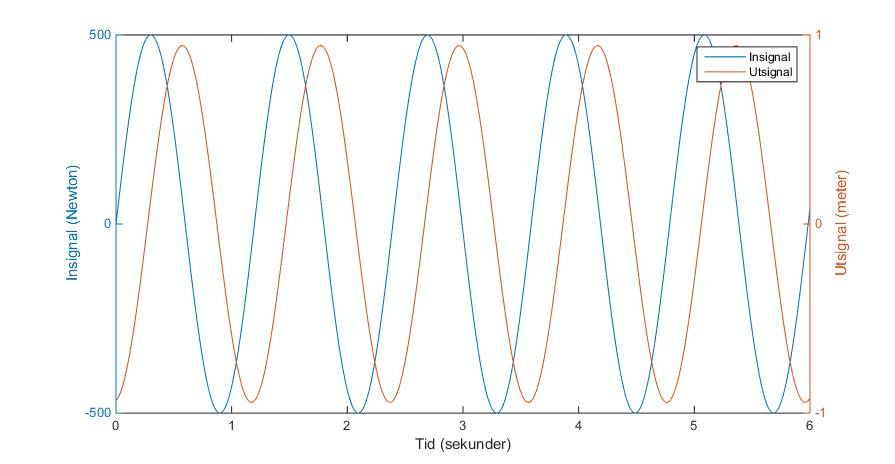
\includegraphics[scale=0.4]{sinussvar1}
\caption{Resonansfrekvens}
\end{center}
\end{figure}

Det intresanta för oss är amplitudskalningen. Vi kan se att den är $0,94$ med andra ord så får vi en amplitud på 0.94 meter. För att trycka ifrån med 500 newton och hoppa i resonansfrekvens ser vi detta som ett rimligt värde.

Vi vill sedan testa om vi har en mycket mycket låg amplitud i vårt fall väljer vi $\omega_0 = 1,5$ som ger:

\begin{equation}
y(t) = 0,27 sin(1,5 t - 0,08)
\end{equation}

\begin{figure}[h]
\begin{center}
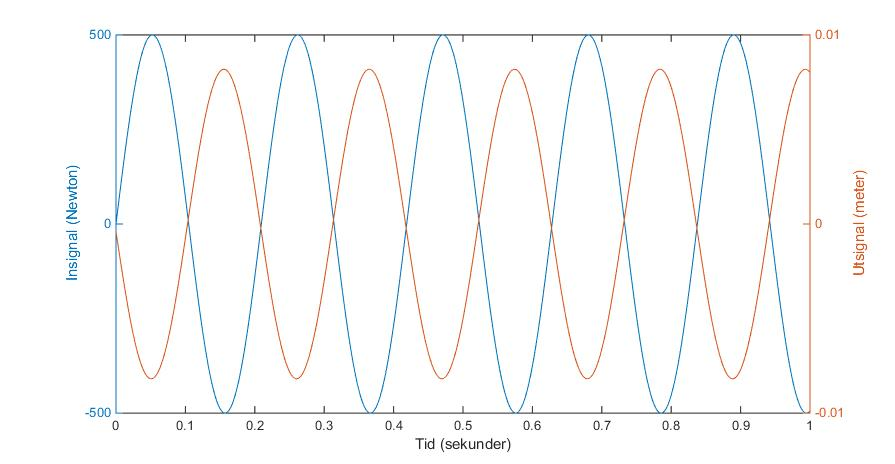
\includegraphics[scale=0.4]{sinussvar2}
\caption{Låg frekvens}
\end{center}
\end{figure}

\newpage
Vi ser att vi får en amplitud som ligger runt 0,27 meter vilket är rimligt då vi trycker med en kraft $500N$ och har en fjäderkonstant på $2000$ Vi får i princip bara $500/2000 = 0,25$. Vi får dock ett litet tillslag för att vi har en frekvens om än låg.

För vår sista sinus har vi valt en hög frekvens $\omega_0 = 30$ som ger:

\begin{equation}
y(t) = 8\cdot 10^{-3} sin(30 t - 3.09)
\end{equation}

\begin{figure}[h]
\begin{center}
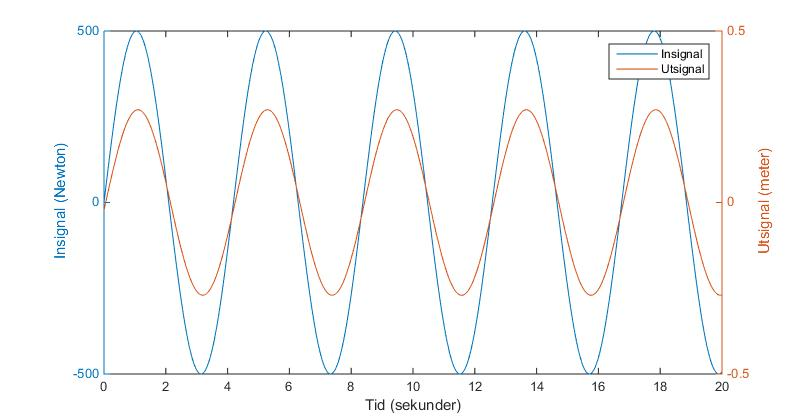
\includegraphics[scale=0.4]{sinussvar3}
\caption{Hög frekvens}
\end{center}
\end{figure}

Vi ser att vi får en mycket mycket liten amplitud vilket är realistiskt för en hög frekvens.




\newpage
\section{Variationer av systemet}

I det här kapitlet kommer vi att visa vad som händer med vårt system om man varierar olika parametrar. Vi kommer svara på frågor som hur studsmattans egenskaper blir annorlunda för en person med en annan vikt, hur olika dämpningar påverkar studsmattan och vad som händer om man har starkare eller svagare fjädrar.



\subsection{Variation av massan}

Om massan hos den hoppande personen ändras så påverkas amplitud och fas-karaktäristiken för systemet. Detta kommer att påverka flera saker för den som hoppar. Figur 18 visar hur vår amplitud och fas-karaktäristik ser ut när vi stoppar in andra värden för massan. 

\begin{figure}[h]
\begin{center}
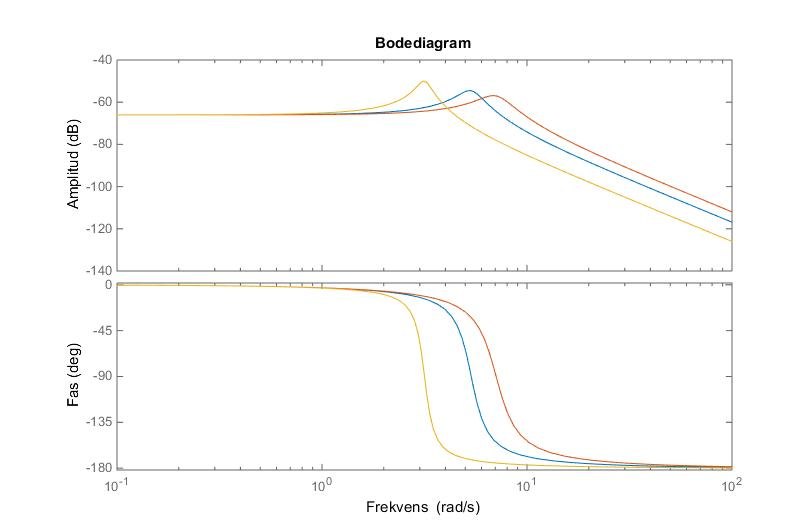
\includegraphics[scale=0.5]{Bode(massa)}
\caption{Bodediagram med 3 olika massor}
\end{center}
\end{figure}

Vi ser att en större massa ger ett större maxvärde för amplituden. Detta innebär att en tyngre person kan i vårt system gunga högre med samma kraft än vad en lättare person skulle kunna göra. Vi ser även att den maximala amplituden sker vid en lägre frekvens för högre massor än för lägre massor. Vi kan även avläsa att lägre massor har ett lite större spektrum utav frekvenser där de får rimlig amplitud då de klarar sig bättre för högre frekvenser

\newpage

\begin{figure}[h]
\begin{center}
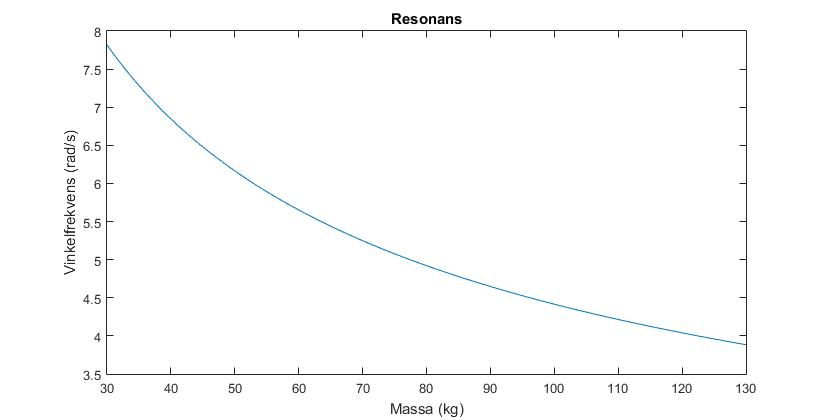
\includegraphics[scale=0.4]{resonans}
\caption{Resonansvinkelfrekvensen som en funktion av massan.}
\end{center}
\end{figure}


Vi kan ur figur 19 avläsa att en högre massa ger en lägre resonansfrekvens och en lägre massa ger en högre resonansfrekvens. Detta innebär att en tyngre person hoppar med lägre frekvens men högre och en lättare person hoppar med en högre frekvens men inte lika högt. Detta är rimligt då dämpningskraften kan retardera systemet mer då massan är lägre och att kraften kan retardera mindre om massan är högre. Fjädern måste sträckas ut mer för en tyngre person så den tyngre personen tillryggalägger mer sträcka per period, det betyder att varje period kommer att ta längre tid. Dock så kommer inte skillnaden att vara jättestor då den tyngre personen färdas snabbare under den extra sträckan. Detta resulterar i att en tyngre person gungar med en lägre frekvens än en lättare person.

\subsection{Variation av dämpningskonstant}

Man kan få studsmattan att bete sig mycket annorlunda genom att ändra på dämpningskonstanten. Vi har valt att analysera hur systemet ändrar sig för en mycket lägre dämpningskonstant, samt vad som händer då man väljer en mycket högre dämpningskonstant så att systemet blir överdämpat. Om vi justerar våra värden så får vi graferna i figur 20.

\newpage

\begin{figure}[h]
\begin{center}
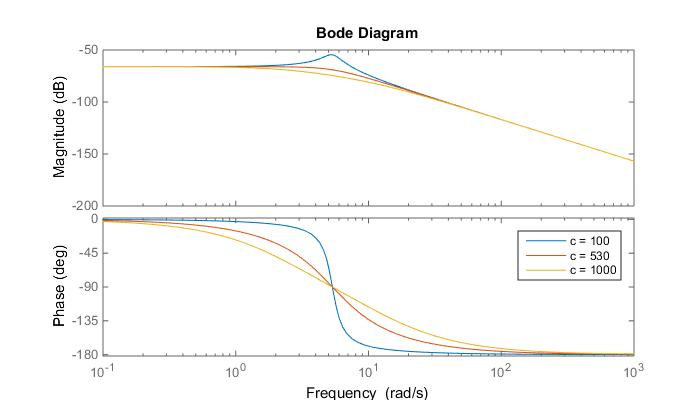
\includegraphics[scale=0.5]{Bode(dampning)}
\caption{Bodediagram för tre olika dämpningar}
\end{center}
\end{figure}

Vi kan se att systemet oscillerar mer om man har en lägre dämpningskonstant. Detta är för att dämpninngen är det som bromsar systemet och gör så att energin läcker ut. Vi vill undersöka vad som händer med resonansfrekvensen för olika dämpningskonstanter. Figur 21 visar resonansfrekvensen för olika dämpningskonstanter för vårt system.

\begin{figure}[h]
\begin{center}
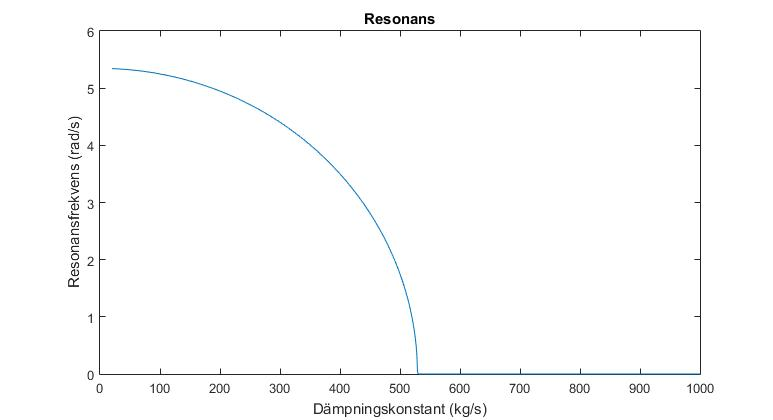
\includegraphics[scale=0.4]{resonansDamp}
\caption{Resonansvinkelfrekvensen som en funktion av dämpningskonstanten.}
\end{center}
\end{figure}

I figur 21 återfinner vi ett annat intressant fenomen. Frekvensen minskar såsom dämpningen ökar, men vid c.a. $530\frac{kg}{s}$ slår den i botten och sedan är resonansfrekvensen $0$. Detta beror på att vi där har nått kritisk dämpning (och därefter överdämpning) och således inte kan få någon självsvängning. Detta sker när systemet dämpar kraften så pass mycket att utsignalen aldrig tar sig över jämnviktsläget. Det skulle hos en studsmatta innebära att man bara sjunker ner i mattan och inte får någon kraft tillbaka uppåt.

\subsection{Variation av fjäderkonstanten}


\begin{figure}[h]
\begin{center}
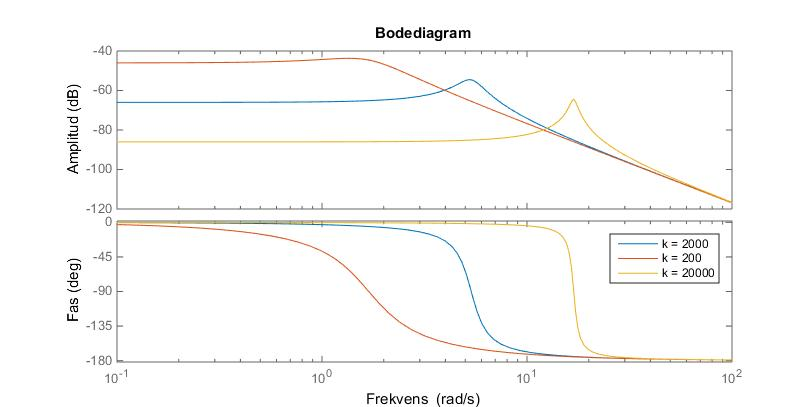
\includegraphics[scale=0.5]{Bode(fjader)}
\caption{Bodediagram för tre olika fjäderkonstanter}
\end{center}
\end{figure}

I figur 23 ser vi att resonansfrekvensen blir högre med fjäderkonstanten. Med andra ord kommer frekvensen att gå ned då fjädrarna blivit lite slitna och rostiga efter några år av slitage. Detta verkar också rimligt.

\begin{figure}[h]
\begin{center}
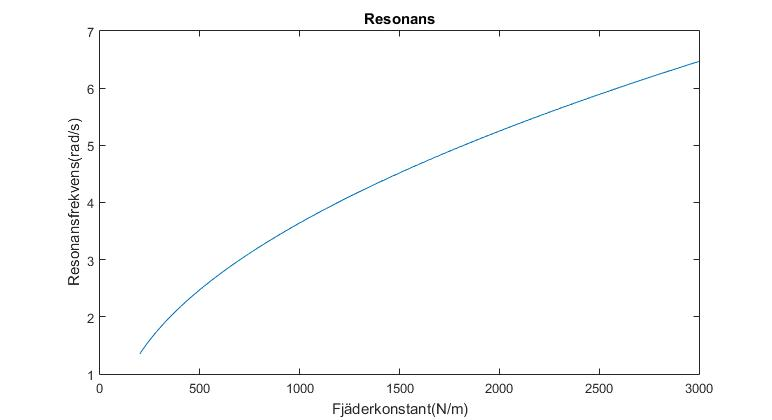
\includegraphics[scale=0.4]{resonansFjader}
\caption{Resonansvinkelfrekvensen som en funktion av fjäderkonstanten.}
\end{center}
\end{figure}



\section{Diskussion}

\subsection{Idealisering}
Systemet som vi modellerar är en studsmatta som vi har idealiserat på olika sätt för att ta fram vår specifika model och för att kunna betrakta det som ett stabilt-LTI system. Dessa idealiseringar betyder självklart att modellen vi har räknat på inte är lika komplex som en studsmatta faktiskt är. 

Det finns en stor mängd mindre relevanta skillnader mellan en verklig studsmatta och vår modell, t.ex. att en person inte hoppar helt centralt i mittpunkten på studsmattan. Vi tänker inte diskutera dessa här utan fokusera på de större avikelserna.

En studsmatta är konstruerad så att den släpper igenom så mycket luft som möjligt när den rör på sig. Men att man måste flytta på luft och att det skapar luftmotstånd kommer man inte ifrån. Detta är en relevant skillnad mellan det mer komplexa fallet av en riktig studsmatta och vår modell. Man kan dock mycket smidigt säga att luftmotståndet bidrar till dämpningen eftersom att det retarderar mattan. I verkligheten kommer den inte att göra detta linjärt men det kan vi se som en mindre avvikelse och säga att luftmotståndet i stort tas hänsyn till genom vår dämpningskonstant.

Den förmodligen mest relevanta skillnaden mellan vår modell och en riktig studsmatta är att när man hoppar på en riktig studsmatta så lämnar man mattan med sin kropp och flyger upp i luften för att sedan landa på mattan igen. Detta betyder att fjäderkraften inte drar tillbaka massan mot marken utan bara drar den uppåt medan gravitationskraften är den enda externa kraften som drar ner massan till studsmattan igen. I vår modell därimot så modellerar vi det som att en person står med fötterna fastspända på mattan, det betyder att fjäderkraften alltid kommer att dra med en kraft neråt på massan då vi är ovanför vårt jämnviktsläge.

Vidare hinner en verklig studsmatta i princip gå tillbaka till sitt jämnviktsläge medan hopparen är i luften, för att sedan påverkas av en mycket stor kraft när denne landar. Så funkar inte vår modell.

Detta har flertalet efterverkningar på vårt system, en av de större effekterna är att vi får en annan resonansfrekvens än vad som skulle vara fallet när man hoppar på en riktig studsmatta. Vi kan se att resonansfrekvensen vi får fram för vårt system är högre än frekvensen hos en person som hoppar på en studsmatta vilket då är rimligt p.g.a att vi har den extra fjäderkraften som drar ner studsmattan mot marken igen och som ökar frekvensen.

\subsection{Vad som har analyserats och varför}

I denna rapport har vi tagit fram en rad systemegenskaper som vi anser vara relevanta för att studera vårt system. Vi har tagit fram systemfunktionen då den låter oss ta fram pol-nollställe diagram och i ävrigt ger mycket information om systemet. Systemfunktionen använder vi även som bas för att få fram vår frekvensfunktionen som ger oss vår  amplitudkaraktäristik och faskaraktäristik. Dessa säger mycket om hur våra utsignaler kommer se ut för olika insignaler. Ett exempel på detta är att de bestämmer vilken variation av en sinusformad insignal vi får som utsignal

Vi tog fram impulssvaret som fungerar som en bas för att ta fram både stegsvaret och stabilitetsbeviset. Stegsvaret ger oss information om hur studsmattan skulle reagera om en person hoppade på studsmattan och hur den svänger in sig till sitt nya jämnviktsläge. En annan tolkning kan vara att en person redan står på studsmattan och fångar en massa och stegsvaret visar hur studsmattan ocillerarar in till sitt nya jämnviktsläge.

\subsection{Vad som inte har analyserats och varför}

En sak man ofta vill analysera för system av liknande stystem är ett rampsvar. Med det avses vad som händer vid en konstant stigande insignal. Detta skulle kunna vara relevant om man modellerar med t ex en lägesändring som insignal och en annan lägesändring som en utsignal. I detta fall kan ett rampsvar representera t.ex. hur en bils fjädring beter sig då bilen kör upp för en backe. I vårt fall har vi dock en kraft som insignal och vi ansåg inte att en analys av en konstant stigande kraft som insignal skulle vara en relevant analys.

I vårt system skulle ett rampsvar kunna tolkas som att en person står på en studsmatta och håller i en jättestor tom bägare som fylls med ett konstant flöde av vatten. Rampsvaret skulle då visa hur studsmattans lägesändring såg ut i detta fal. Vi ansåg inte att detta var en relevant analys utav en studsmattas egenskaper och kan inte direkt kopplas till syftet eller målet med vår rapport, så vi valde att inte göra en sådan analys även om resultatet skulle kunna vara intressant. Värt att notera är att man skulle kunna tolka det som att en personen som hoppar trycker ifrån mer och mer under en mycket kort tidsperiod. Vi väljer att tolka problemet som att en person trycker ifrån med en konstant kraft.




\newpage

\begin{thebibliography}{9}

\bibitem{sune2000}
  Sune Söderkvist,
  \emph{Tidskontinuerliga Signaler \& System}.
  \newline
  Erik Larsson AB, Linköping,
  3e upplagan,
  2000.
  
\bibitem{randall2008}
	Randall D. Knight,
	\emph{Physics for Scientists and Engineers: A Strategic Approach with Modern Physics (2nd Edition)}.
	\newline
Addison-Wesley, 2a upplagan, 2008.

\bibitem{polesAndZeros}

	\emph{Understand Poles and Zeros}.
	\newline
	Publicerad 2002-11-01. Hämtat: 2015-06-01.
	\newline
	URL: http://web.mit.edu/2.14/www/Handouts/PoleZero.pdf

\end{thebibliography}


\newpage

\section{Komplettering}



\subsection{Jämviktsläget}

I vår rapport så tar vi upp jämviktsläget ganska kort när vi förklarar de krafter som påverkar systemet och hur vi räknar på utsignalen. Vi fick kommentaren att jämviktsläget är otydligt från figuren. I orginalbilden utgick alla kraftpilar från studsmattans kant ("grundläge") även fast en person stod på mattan. Dessutom var varken studsmattans grundjämviktsläge eller nya jämviktsläget med massan på markerade. Dessa brister är redigerade i ((figur X)). 

((((FIGUR))))

Dessutom kunde vi ha varit tydligare i texten med hur vi betecknade de olika jämviktslägena och avvikelsen. Till en början använde vi $L$ som grundjämviktsläget (d.v.s. om ingen massa är på mattan), $l_1$ som det nya jämviktsläget med en massa på och $l_0$ som avvikelsen. Eftersom avvikelsen kan vara både nedåt (positiv riktning) och uppåt (negativ riktning) så blir det lite klumpigt att bara använda en sträcka eftersom den inte kan vara negativ. Kan då vara bättre att använda $\Delta l$ som avvikelsen från grundjämviktsläget.

\subsection{Differentialekvationen}

Med de påverkade krafterna i systemet $F_a = x(t), F_g = mg, F_f = -k(\Delta l + y(t),F_d = -cv$ och med Newtons andra lag fick vi fram ekvationen:
\begin{equation}
F_tot = x(t) + mg - k(\Delta l + y(t)) - cv = ma
\end{equation} 
Där $x(t)$ är insignalen, $y(t)$ är utsignalen, $k$ är fjäderkonstanten, $c$ är dämpningskonstanten, $m$ är personen på mattans massa, $v$ är hastigheten, $a$ är accelerationen och $g$ är gravitationen. Om vi då uttrycker acceleration och hastighet som funktioner av tiden så kan vi uttrycka en differentialekvation.
\begin{equation}
a = \frac{d^2y(t)}{dt^2} , v = \frac{y(t)}{dt}
\end{equation}
Vilket ger:
\begin{equation}
 m\frac{d^2y(t)}{dt^2} =  -k(\Delta l + y(t)) -c\frac{dy(t)}{dt} + mg +  x(t)
\end{equation}

I det sista steget för den slutgiltiga differentialekvationen så fick vi kommentaren att vi skulle visa ett steg mer matematiskt. Vi skrev kort och gott att vid tid $t = 0$ så kommer gravitationen och fjäderkraften som verkar på massan ta ut varandra, och därav befinna sig i jämvikt.

För att detta ska vara tillräckligt bör vi visa hur detta kommer sig. Vi kan visa detta genom att utgå från ekvation ((X)).
\begin{equation}
\begin{split}
 m\frac{d^2y(t)}{dt^2} =  -k(\Delta l + y(t)) -c\frac{dy(t)}{dt} + mg +  x(t) \\ \leftrightarrow m\frac{d^2y(t)}{dt^2} = x(t) + mg  - k \Delta l -  k y(t)) -c\frac{dy(t)}{dt}  
\end{split}
\end{equation}
Om vid $t = 0$ både insignal $x(0) = 0$ och utsignal $y(0) = 0$ så får vi bara kvar
\begin{equation}
0 = mg  - k \Delta l
\end{equation}
Om vi stoppar in detta samband i ekvation ((X)) så får vi vår slutgiltiga differentialekvation:
\begin{equation}
\begin{split}
m\frac{d^2y(t)}{dt^2} = x(t) + mg  - k \Delta l -  k y(t)) -c\frac{dy(t)}{dt} \\ \leftrightarrow
 m\frac{d^2y(t)}{dt^2} + k  y(t) + c\frac{dy(t)}{dt} = x(t)
 \end{split}
\end{equation}

\subsection{Val av konstanter}

Vårt val av konstanter blev lite hastigt och förklarades inte. Vi fick därav kommentaren att vi borde motivera dem. 

\subsection{Laplacetransform}

\subsection{Stabilitetsbevis}

\subsection{Frekvensfunktion}

\subsection{Impuls- och stegsvar för olika system}

\end{document}